\documentclass[11pt,a4paper]{article}
\usepackage{hyperref}
\usepackage[margin=2.5cm]{geometry}
\usepackage{amsmath, amsthm}
\usepackage{txfonts}
\usepackage{todonotes}
\usepackage{enumitem}
\usepackage{listings}
\usepackage[nameinlink]{cleveref}
\usepackage{microtype}
\usepackage{algorithm}
\usepackage{algpseudocode}
\usepackage{tikz}

\hypersetup{
  pdftitle={Storing the Cardano ledger state on disk},
  pdfborder={0 0 0},
  breaklinks=true
}

\usetikzlibrary{arrows.meta}
\usetikzlibrary{intersections}

% https://tex.stackexchange.com/questions/229940/can-i-have-a-listing-with-fixed-column-code-and-full-flexible-comments
\makeatletter
\let\commentfullflexible\lst@column@fullflexible
\makeatother

\makeatletter
\tikzset{
    database/.style={
        path picture={
            \draw (0, 1.5*\database@segmentheight) circle [x radius=\database@radius,y radius=\database@aspectratio*\database@radius];
            \draw (-\database@radius, 0.5*\database@segmentheight) arc [start angle=180,end angle=360,x radius=\database@radius, y radius=\database@aspectratio*\database@radius];
            \draw (-\database@radius,-0.5*\database@segmentheight) arc [start angle=180,end angle=360,x radius=\database@radius, y radius=\database@aspectratio*\database@radius];
            \draw (-\database@radius,1.5*\database@segmentheight) -- ++(0,-3*\database@segmentheight) arc [start angle=180,end angle=360,x radius=\database@radius, y radius=\database@aspectratio*\database@radius] -- ++(0,3*\database@segmentheight);
        },
        minimum width=2*\database@radius + \pgflinewidth,
        minimum height=3*\database@segmentheight + 2*\database@aspectratio*\database@radius + \pgflinewidth,
    },
    database segment height/.store in=\database@segmentheight,
    database radius/.store in=\database@radius,
    database aspect ratio/.store in=\database@aspectratio,
    database segment height=0.1cm,
    database radius=0.25cm,
    database aspect ratio=0.35,
}
\makeatother

\lstset{
  language=haskell
  , basicstyle=\small\ttfamily
  , keywordstyle=\bfseries
  , commentstyle=\normalsize\rmfamily\itshape\commentfullflexible
  , columns=fixed
  , morekeywords={
    family
    , Type
  }
}

\theoremstyle{definition}
\newtheorem{property}{Property}
\newtheorem{definition}{Definition}
\newtheorem{lemma}{Lemma}
\newtheorem{assumption}{Assumption}
\newtheorem{corollary}{Corollary}
\newtheorem{proposal}{Proposal}
\newtheorem*{notation}{Notation}
\newtheorem{observation}{Key observation}
\newtheorem{failedattempt}{Failed attempt}

\newenvironment{bug}
  {\begin{quote} \textbf{Known bug}.}
  {\end{quote}}

\title{Storing the Cardano ledger state on disk\\
       {\large \sc UTxO-HD}
  }
\author{The Consensus Team
  }

\newcommand{\debugsep}[1]{
  \vspace{2em}
  \hrule
  \vspace{0.5em}
  \textbf{#1}
  \vspace{0.5em}
  \hrule
  \vspace{2em}
}

% TODO
%
% * Incorporate
%
%   - Previous blog posts
%   - Specifications currently stored as markdown files in the repo
%   - Any discussions in long comments in the code
%
% - choice of k: liveness versus safety
% - make sure we talk about the fact that the ledger can be linear

\newcommand{\duncan}{\todo{Duncan suitable section.}}

\begin{document}

\maketitle

\tableofcontents

\section{Introduction}

The current and first version of UTxO-HD focuses only on moving the UTxO set to
the disk storage. This impacts the Consensus codebase almost in its entirety.
The Ledger and Node layers remain ignorant to this change on their side if the
interface and therefore the consensus side of the interface to them has to be
slightly modified.

The reader is assumed to be familiar with the Consensus report and the general
architecture of the Consensus and Ledger layers.

\section{The LedgerDB}

\subsection{The \texttt{LedgerTables} data family}

As defined in the blockchain literature, a \textbf{Ledger state at block $B$} is
the state of the system after applying all the blocks since Genesis up to block
$B$ (included) on top of the Genesis state. It contains the full state of the
system, namely the UTxO set, the stake delegations, chain state (nonces), etc. A
full description of the Ledger state can be found in the Ledger
specifications\footnote{\href{https://github.com/input-output-hk/cardano-ledger}{https://github.com/input-output-hk/cardano-ledger}}.

As we will be talking about the architectural changes in the code, we will be referring to values of type \texttt{LedgerState blk} as \textbf{Ledger states}.

Previously, a \texttt{LedgerState blk} was a complete representation of the
concept of \textbf{Ledger state} as defined above.

\begin{lstlisting}
type LedgerState :: Type -> Type
data family LedgerState blk
\end{lstlisting}

After UTxO-HD this is no longer the case as the UTxO set has been projected out
of said data-type. The data has then been split between the \emph{in-memory}
part (what we now informally call \emph{the ledger state without tables} or
\emph{the ledger state in memory}) and the \emph{ledger tables} which are
on-disk.

\begin{figure}[h]
  \centering
  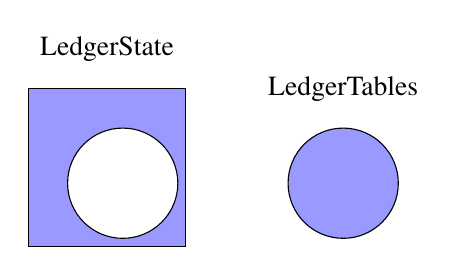
\begin{tikzpicture}
    \filldraw[fill=blue!40!white, draw=black] (0,0) rectangle (2,2);
    \filldraw[fill=white, draw=black] (1.2,0.8) circle (0.7);
    \node at (1,2.5) {LedgerState};
    \filldraw[fill=blue!40!white, draw=black] (4,0.8) circle (0.7);
    \node at (4,2) {LedgerTables};
  \end{tikzpicture}
  \caption{The separation between the ledger state and the tables}
\end{figure}


\begin{lstlisting}
  type MapKind :: {- key -} Type -> {- value -} Type -> Type
  type LedgerStateKind :: MapKind -> Type

  type LedgerState :: Type -> LedgerStateKind
  data family LedgerState

  type LedgerTables :: LedgerStateKind -> LedgerStateKind
  data family LedgerTables
\end{lstlisting}

A ledger state now has ledger tables attached to it, which live outside the
ledger state. The ledger tables represent partial information for the maps that
have been moved to disk, in particular as mentioned above in this version only
the UTxO set. We can access the ledger tables of a ledger state via
\texttt{projectLedgerTables} and we can attach tables to a ledger state via
\texttt{withLedgerTables}.

\begin{lstlisting}
  projectLedgerTables :: l mk  -> LedgerTables l mk
  withLedgerTables    :: l any -> LedgerTables l mk -> l mk
\end{lstlisting}

The tables themselves can represent different logical states of the UTxO set,
either actual values, differences, both or even represent no information about
the UTxO set at all. The alternative values that can be held in the tables are
given by the following GADT:

\begin{lstlisting}
data ApplyMapKind' :: MapKind' -> Type -> Type -> Type where
  ApplyEmptyMK    ::                           ApplyMapKind' EmptyMK'    k v
  ApplyKeysMK     :: !(Set k)               -> ApplyMapKind' KeysMK'     k v
  ApplyValuesMK   :: !(Map k v)             -> ApplyMapKind' ValuesMK'   k v
  ApplyDiffMK     :: !(Map k (DiffEntry v)) -> ApplyMapKind' DiffMK'     k v
  ApplyTrackingMK :: !(Map k v)
                  -> !(Map k (DiffEntry v)) -> ApplyMapKind' TrackingMK' k v
\end{lstlisting}

The intuition about what these values represent can be easily described:
\begin{itemize}
  \item a value of type \texttt{LedgerState blk EmptyMK} can project tables of
        type \texttt{LedgerTables (LedgerState blk) EmptyMK} which holds an
        empty constructor \texttt{ApplyEmptyMK}.
  \item a value of type \texttt{LedgerState blk KeysMK} can project tables of
        type \texttt{LedgerTables (LedgerState blk) KeysMK} which holds a set of
        keys. For the UTxO set case in particular, a set of \texttt{TxIn}s.
  \item a value of type \texttt{LedgerState blk ValuesMK} can project tables of
        type \texttt{LedgerTables (LedgerState blk) ValuesMK} which holds a map
        from keys to values. For the UTxO set case in particular, a map of
        \texttt{TxIn}s to \texttt{TxOut}s.
  \item a value of type \texttt{LedgerState blk DiffMK} can project tables of
        type \texttt{LedgerTables (LedgerState blk) DiffMK} which holds a map
        from keys to diff entries. Diff entries are computed by comparing two
        \texttt{ValuesMK} tables to find out which keys have been
        removed/inserted/updated from one map to another. For the UTxO set case
        in particular, as entries cannot be updated nor they can be inserted
        twice, this holds a map from \texttt{TxIn}s to whether that key was
        inserted (and with what value) or whether it was deleted.
  \item a value of type \texttt{LedgerState blk TrackingMK} can project tables
        of type \texttt{LedgerTables (LedgerState blk) TrackingMK} which is a
        sum of a \texttt{ValuesMK} table and a \texttt{DiffMK} table.
\end{itemize}

The following ghci pseudo-examples show representations of each type of tables:

\begin{lstlisting}
  > let l  = foo :: LedgerState blk EmptyMK
  > let k  = l `withLedgerTables` ApplyKeysMK (fromList [10, 12])
  > let v1 = l `withLedgerTables` ApplyValuesMK (fromList [(0, 0), (1, 1)])
  > let v2 = l `withLedgerTables` ApplyValuesMK (fromList [(1, 1), (2, 4)])
  > printTables l
  Empty
  > printTables k
  ApplyKeysMK   (fromList [10, 12])
  > printTables v1
  ApplyValuesMK (fromList [(0,0), (1,1)])
  > printTables (v2 `diff` v1)
  ApplyDiffMK   (fromList [(0, Delete), (2, Insert 4)])
\end{lstlisting}

\subsection{The discrepancy between in-memory and on-disk}
\begin{observation}
  \emph{The ledger states defined above use \textbf{the same in-memory part} (namely the in-memory part of \texttt{l}).}
  \emph{The part which is not the Ledger tables is unaffected by the particular choice of \texttt{ApplyMapKind}.}
\end{observation}

This is a crucial observation: \texttt{l} is \textbf{not} dependent on the
tables. As mentioned in the beginning of this section, the Ledger interface side
of the Consensus-Ledger interface didn't change so we have to end up providing
data in a structure equivalent to the one before UTxO-HD. In particular, there
must be a field on the data structure hierarchy that builds a
\texttt{LedgerState blk mk} that must contain the UTxO set and nothing prevents
us from having some data there. In particular, the following ledger state is well-shaped:

\begin{lstlisting}
  > let (txin, txout) = ... :: (TxIn blk, TxOut blk)
  > let l' = SomeLedgerStateConstructor {
      .. = {
          ..
        , utxoSet = Map.singleton [(txin, txout)]
        }
      } `withLedgerTables` ApplyEmptyMK :: LedgerState blk EmptyMK
\end{lstlisting}

(Just for simplicity we are assuming \texttt{TxIn} and \texttt{TxOut} depend on
the block type although this is not the case in reality). One can think that
this value makes no sense as it holds a UTxO set despite the tables being empty.
However this comes from the Ledger layer remaining ignorant to UTxO-HD.

The Ledger layer types are wrapped by Consensus types representing the Ledger
state, and despite the tables being part of the latter, they are not part of the
former. As an example, one can see the \texttt{LedgerState (ShelleyBlock proto
  era)} where before UTxO-HD:

\begin{lstlisting}
  data instance LedgerState (ShelleyBlock proto era) = ShelleyLedgerState {
      shelleyLedgerTip        :: !(WithOrigin (ShelleyTip proto era))
    , shelleyLedgerState      :: !(SL.NewEpochState era)
    , shelleyLedgerTransition :: !ShelleyTransition
  }
\end{lstlisting}

The Ledger layer defines \texttt{SL.NewEpochState} (as defined in the Ledger
formal specifications) and the Consensus layer wraps this type in its own
\texttt{LedgerState} data-type instance. Now, after UTxO-HD, this datatype has evolved into the following:

\begin{lstlisting}
  data instance LedgerState (ShelleyBlock proto era) mk = ShelleyLedgerState {
      shelleyLedgerTip        :: !(WithOrigin (ShelleyTip proto era))
    , shelleyLedgerState      :: !(SL.NewEpochState era)
    , shelleyLedgerTransition :: !ShelleyTransition
    , shelleyLedgerTables     :: !(LedgerTables
                                     (LedgerState (ShelleyBlock proto era))
                                     mk)
    }
\end{lstlisting}

The ledger operates with \texttt{NewEpochState}s only so we need some way to move the values on the tables into the UTxO in the \texttt{NewEpochState} and viceversa. Those functions are defined in the class \texttt{StowableLedgerTables}:

\begin{lstlisting}
class StowableLedgerTables l where
  stowLedgerTables   :: l ValuesMK -> l EmptyMK
  unstowLedgerTables :: l EmptyMK  -> l ValuesMK
\end{lstlisting}

So now, using the same values as in previous code snippets:
\begin{lstlisting}
  > printUtxosInNewEpochState l'
  fromList [(txin, txout)]
  > printTables l'
  Empty
  > printTables (unstowLedgerTables l')
  ApplyValuesMK (fromList [(txin, txout)])
  > printUtxosInNewEpochState (unstowLedgerTables l')
  fromList []
  > stowLedgerTables (unstowLedgerTables l') == l'
  True
\end{lstlisting}

Note that the hole left by extracting the tables is not really a hole as
pictured earlier in this section, but instead it is filled with an empty
\texttt{Data.Map} container.


\begin{observation}
  \label{ko1}
  \emph{The only way to mimick a full ledger state is by holding a initial set
    of values and a sequence of differences}.
\end{observation}

\subsection{Notation}
When representing a ledger state from now on, in case the ledger state is as
known by the ledger (oblivious to ledger tables), we will denote it with
$\mathbb{L}$, and otherwise we will denote it as $L^{s}_{T}$ where $s$ means the
slot to which the ledger state was ticked and $T$ the tables attached to this
ledger state. Note that in particular $L_{E}$ can always be seen as $\mathbb{L}$.

\subsection{In memory design}

The ledger database was traditionally made of \texttt{AnchoredSeq}s of ledger
states, but as of UTxO-HD this is no longer the case. We hold
\texttt{AnchoredSeq}s of \emph{in-memory} ledger states and the corresponding
sequence of differences to the tables. This is perfectly shown by the
\texttt{DbChangelog} datatype:

\begin{lstlisting}
data DbChangelog l = DbChangelog {
    changelogDiffAnchor      :: !(WithOrigin SlotNo)
  , changelogDiffs           :: !(LedgerTables l SeqDiffMK)
  , changelogImmutableStates ::
      !(AnchoredSeq
          (WithOrigin SlotNo)
          (DbChangelogState l)
          (DbChangelogState l)
       )
  , changelogVolatileStates  ::
      !(AnchoredSeq
          (WithOrigin SlotNo)
          (DbChangelogState l)
          (DbChangelogState l)
       )
  }
\end{lstlisting}

The sequence of differences held in the \texttt{DbChangelog} correspond to the
differences produced when going from one of the states in the fragments to the
next one, i.e. the first map of differences belongs to the differences produced
when applying the first block which produced the first element in the sequence
of states, and so on.

There is one important observation here: the sequence of differences is relative
to some initial (or anchor) set of values. This set of values lives in the disk
and is what will be refered as the \textbf{Backing store} from now on. It
represents the UTxO values at the ledger state referenced as the anchor of the
sequence of immutable states.

\begin{figure}[h]
  \centering
  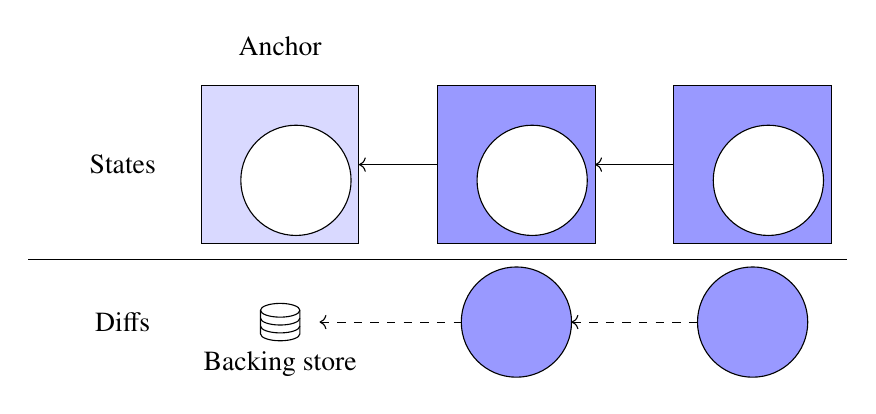
\begin{tikzpicture}
    \node at (-1,1) {States};
    \node at (1,2.5) {Anchor};
    \draw (-2.2,-0.2) -- (8.2,-0.2);
    \filldraw[fill=blue!15!white, draw=black] (0,0) rectangle (2,2);
    \filldraw[fill=white, draw=black] (1.2,0.8) circle (0.7);
    \draw[<-] (2,1) -- (3,1);
    \filldraw[fill=blue!40!white, draw=black] (3,0) rectangle (5,2);
    \filldraw[fill=white, draw=black] (4.2,0.8) circle (0.7);
    \draw[<-] (5,1) -- (7,1);
    \filldraw[fill=blue!40!white, draw=black] (6,0) rectangle (8,2);
    \filldraw[fill=white, draw=black] (7.2,0.8) circle (0.7);

    \filldraw[fill=blue!40!white, draw=black] (4,-1) circle (0.7);
    \filldraw[fill=blue!40!white, draw=black] (7,-1) circle (0.7);
    \node at (-1,-1) {Diffs};
    \node[database,label=below:Backing store] at (1, -1){};
    \draw[<-,dashed] (1.5,-1) -- (3.3,-1);
    \draw[<-,dashed] (4.7,-1) -- (6.3, -1);
  \end{tikzpicture}
  \caption{The DbChangelog} \label{fig:dbch}
\end{figure}

Before UTxO-HD, pruning the ledger database was done just by dropping items from
the beginning of the sequence of immutable states. However, now we need to also
flush their corresponding differences into the backing store in order to keep
both sides of the DbChangelog in sync.

Furthermore, we cannot perform this operation at will, as we could fall into
inconsistent states. As described in \textbf{Key observation \ref{ko1}}, in
order to preserve the consistency needed to mimick a complete ledger state there
will be moments in which we cannot let the Ledger database perform side effects
on the backing store.

\begin{observation}
  \label{ko2}
  \emph{Whenever we acquire a LedgerState on top of which we plan to apply
    transactions (or blocks) for which we still don't have forwarded the tables
    of values, we need to also acquire the corresponding DbChangelog and hold
    the flush lock in read mode}.
\end{observation}

\subsection{Backing store definition and implementations}

\begin{definition}
  The \textbf{backing store} is some stateful storage which holds the UTxO
  values as of some block in the immutable database. It is unique, i.e. there is
  only one in the system.
\end{definition}

It has to support essentially:

\begin{itemize}
  \item \textbf{WRITE}: Update of values.
  \item \textbf{READ}: Temporary consistent views of values for querying.
  \item \textbf{SNAPSHOT}: Persistent copies used when restarting the node.
\end{itemize}

The way we ensure that there will never be rollbacks and that we using a
changelog in sync with the backing store is by keeping a \emph{sequence number}.
Note that rollbacks can't happen as we only flush changes that belong to
immutable states.

\subsubsection{InMemory}

The \texttt{InMemory} implementation is a super straightforward implementation
of the concept of the backing store. It is essentially a \texttt{TVar} holding a
\texttt{Data.Map} of keys to values. The operations are achieved as follows:

\begin{itemize}
  \item \textbf{WRITE}: Just a normal update on a \texttt{Data.Map}.
  \item \textbf{READ}: Just a normal read on the \texttt{TVar} provides a \texttt{Data.Map}.
  \item \textbf{SNAPSHOT}: Serializing the contents of the \texttt{Data.Map} into some file.
\end{itemize}

The sequence number is kept alongside the \texttt{Data.Map}.

\begin{lstlisting}
data TVarBackingStoreContents m values =
     TVarBackingStoreContentsClosed
   | TVarBackingStoreContents
      !(WithOrigin SlotNo)
      !values
\end{lstlisting}

\subsubsection{LMDB}

The LMDB\footnote{http://www.lmdb.tech/doc/} implementation uses a key-value store on the disk and things get somewhat more complicated. The operations are achieved as follows:

\begin{itemize}
  \item \textbf{WRITE}: LMDB provides an API function for inserting/updating/deleting values.
  \item \textbf{READ}: Holding onto a \emph{read} LMDB transaction provides a
        consistent view of the database for as long as the transaction is kept
        open.
  \item \textbf{SNAPSHOT}: LMDB provides an API function to copy a whole
        database onto a separate directory.
\end{itemize}

The data is essentially split in two tables, namely \emph{dbState} (which
holds the sequence number explained above), and a table with a name
dictated by the actual block type in use by the node.

\subsubsection{LSM Trees}

TBD

\section{Interface with the Ledger}

The Ledger layer has not been modified for UTxO-HD and therefore the ledger
states that we provide to the ledger must be indistinguishable from those before
UTxO-HD in what matters to the Ledger rules that will be executed. In order to
understand why some actions are allowed, one has to interiorize the following
\textbf{Key observations}:

\begin{observation}
  \emph{In order to succesfully apply a block, the UTxO set inside the ledger state
  only needs to contain the entries requested by the transactions in the block.}
\end{observation}

This is also true when speaking about transaction application: only the inputs
requested by the transaction are actually needed by the Ledger.

\begin{observation}
  \emph{In order to succesfully tick a block not through an era transition, the
    UTxO set can be empty as the ledger rules don't look at it.}
\end{observation}

\begin{observation}
  \emph{Ticking through an era transition might require some entries on the UTxO set
  and can produce changes in them.}
\end{observation}

It is precisely by this last observation, that ticking has to be considered as
producing tables with differences.

The sequence of actions for ticking and applying a block $B$ at slot $s$ on top
of a ledger state $L$ is then easily described by \textbf{Algorithm \ref{alg:tickandapply}}.

\begin{algorithm}[h]
  \caption{Tick and apply}
  \label{alg:tickandapply}
  \begin{algorithmic}[1]
    \Procedure{TickAndApply}{$DB :: \texttt{LedgerDB}, B :: \texttt{Block}$}
    \State $L_{E} \gets \texttt{getLedger}_{DB}(\texttt{Pred}(B))$
    \State $\mathbb{L}^{s} \gets \texttt{TICK}(\mathbb{L}, s)$ \Comment{Note that $\mathbb{L} \eqsim L_{E}$}
    \State $\texttt{Diffs}_{s} \gets \texttt{diff}(\mathbb{L}^{s}, \mathbb{L})$
    \Statex
    \State $V_{in} \gets \texttt{queryDisk}_{DB}(\texttt{keySets}(B)) \triangleleft \texttt{Diffs}_{DB}(\texttt{Pred}(B)) \triangleleft \texttt{Diffs}_{s}$ \Comment{$\triangleleft$ means \textbf{forward}}
    \Statex
    \State $\mathbb{L}^{s}_{[V_{in}]} \gets \texttt{stowLedgerTables}(L^{s}_{{V_{in}}})$
    \State $\mathbb{L}' \gets \texttt{APPLY}(B, \mathbb{L}^{s}_{[V_{in}]})$
    \State $\texttt{Diffs}_{B} \gets \texttt{diff}(\mathbb{L}', \mathbb{L}^{s}_{[V_{in}]})$
    \Statex{}
    \State \Return $L'_{(\texttt{Diffs}_{s}~\diamond~\texttt{Diffs}_{B})}$
    \EndProcedure
 \end{algorithmic}
\end{algorithm}

where \texttt{queryDisk} means consulting the Backing store and $\texttt{Diffs}_{DB}(Z)$ are the current diffs in the LedgerDB up to the requested block $Z$.

\section{Anti-diffs}

\subsection{The FingerTree problem}

\subsection{Algebra of differences}

\subsection{It is a semigroupoid!}

\section{The Mempool}

\subsection{Definition and design}

In the Cardano node, the mempool plays a central role when forging the chain. Citing from the report:
\begin{quote}
  Whenever a block producing node is the leader of a slot, it gets the chance to
  mint a block. For the Cardano blockchain to be useful, the minted block in the
  blockchain needs to contain \emph{transactions}. The mempool is where we buffer
  transactions until we are able to mint a block containing those transactions.
\end{quote}

We can consider the mempool as a stateful ubiquitous container that is accessed
from multiple places at the same time and should be able to provide a list of
transactions which are valid on top of a given state. And if possible, it should
try to add transactions on top of the best known ledger state so that in the
event that we need to forge on top of it, we don't need to revalidate all the
transactions (or at least most invalid transactions have already been
discarded). The interface to the mempool is roughly as follows:

\begin{lstlisting}
data Mempool m blk idx = Mempool {
   tryAddTxs      :: WhetherToIntervene
                  -> [GenTx blk]
                  -> m ( [MempoolAddTxResult blk]
                       , [GenTx blk]
                       )
 , syncWithLedger :: m (MempoolSnapshot blk idx)
 , getSnapshotFor :: SlotNo
                  -> TickedLedgerState blk DiffMK
                  -> MempoolChangelog blk
                  -> m (MempoolSnapshot blk idx)
 , ...
}
\end{lstlisting}

At every point in time, the mempool is anchored on top of the best ledger state
known by the ChainDB, and a background thread is in charge of making sure that
whenever the tip of the chain changes, the mempool gets revalidated.

The mempool holds a \emph{virtual ledger state} resulting from ticking the
anchor ledger state to some preemptive slot number and then applying all the
currently valid transactions on top of it. Now that UTxO-HD has redefined what a
ledger state is, the mempool holds not only a virtual ledger state but also a
view on the sequence of differences that would correspond to that ledger state.
This is shown by the data held in the Mempool's \texttt{InternalState}:

\begin{lstlisting}
data InternalState blk = IS {
   -- | Transactions currently in the mempool
   isTxs          :: !(TxSeq (Validated (GenTx blk)))

   -- | The cached ledger state after ticking the ledger state identified by
   -- 'isTip' to 'isSlotNo' and applying the transactions in the Mempool
   -- against this ledger state. New transactions will be validated by
   -- applying them on top of 'isLedgerState'.
 , isLedgerState  :: !(TickedLedgerState blk TrackingMK)

   -- | The changelog as captured on the last sync with the ledger.
 , isDbChangelog  :: !(MempoolChangelog blk)
   ...
}
\end{lstlisting}

This internal state is kept inside a \texttt{StrictTMVar} by the
\texttt{MempoolEnv} and the different operations on the mempool have to make
sure that there is no path in which the \texttt{TMVar} would remain empty (and
therefore produce a lock). It is important to note that this has to be a
\texttt{TVar} because concurrent addition of transactions have to be done in
atomic steps, and it has to be a \texttt{MVar} because we need to perform
\texttt{IO} while the contents must remain non-updateable by other actors.

In particular, most of the operations on the mempool follow this pattern:

\begin{algorithm}
  \caption{Pattern of mempool operation}
  \begin{algorithmic}[1]
    \Procedure{MempoolOp}{$M :: \texttt{Mempool}$}
    \State $\texttt{is} \gets \texttt{atomically} (\texttt{takeTMVar}_{M}) $
    \State $x \gets \texttt{someIO}(\texttt{is})$
    \State $\texttt{atomically}(\texttt{doSomething}(x) >>= \texttt{putTMVar}_{M})$
    \EndProcedure
 \end{algorithmic}
\end{algorithm}

The \texttt{someIO} is usually consulting the Backing store for UTxO values, and
then \texttt{doSomething} is the actual operation that we want to perform more
or less as it was done before UTxO-HD.

\subsection{Operations}

\subsubsection{Adding transactions}

The problem of applying transactions is then solved in a very straightforward
way, quite similarly to applying a block:

\begin{algorithm}
  \caption{Adding a transaction}
  \begin{algorithmic}[1]
    \Procedure{TryAddTx}{$DB :: \texttt{LedgerDB}, M :: \texttt{Mempool}, tx :: \texttt{Tx}$}
    \State $L_{\texttt{Diffs}_{M}} \gets \texttt{isLedgerState}_{M}$
    \State $V_{in} \gets \texttt{queryDisk}_{DB}(\texttt{keySets}(tx)) \triangleleft \texttt{isDbChangelog}_{M} \triangleleft \texttt{Diffs}_{M}$
    \If {\texttt{isError}($V_{in}$)}
    \State $M' \gets \texttt{SyncWithLedger(DB,M)}$
    \State $\texttt{TryAddTx}(DB,M',tx)$
    \Else
    \State $\mathbb{L}^{s}_{[V_{in}]} \gets \texttt{stowLedgerTables}(L_{V_{in}})$
    \State $\mathbb{L}' \gets \texttt{APPLY}(tx, \mathbb{L}^{s}_{[V_{in}]})$
    \If {\texttt{isError}($\mathbb{L}'$)}
    \State \Return $M$
    \Else
    \State $\texttt{Diffs}_{tx} \gets \texttt{diff}(\mathbb{L}', \mathbb{L}^{s}_{[V_{in}]})$
    \State \Return $M [ \texttt{isLedgerState} \mapsto L'_{\texttt{Diffs}_{M}~\diamond~\texttt{Diffs}_{tx}}, \texttt{isTxs} \mapsto tx: \texttt{isTxs}_{M}]$
    \EndIf
    \EndIf
    \EndProcedure
 \end{algorithmic}
\end{algorithm}

The resulting ledger state is stored in the Mempool's internal state and the
transaction is added to the list of valid transactions. Of course, in the same
way as before UTxO-HD, when the transaction fails to apply, the result is
discarded.

This process mimicks the process before UTxO-HD in which the mempool held a
complete ledger state with the whole UTxO set in it and applied transactions to
it. Now only one more special case arises which was not needed prior to these
changes: the disk anchor moving.

If \texttt{queryDisk} fails to retrieve the values because the
\texttt{DbChangelog} held by the mempool got out of sync with the one on the
disk, we are forced to perform a sync with the ledger in order to get an up to
date \texttt{DbChangelog}. As the anchor belongs to the immutable part of the
ledger database, it can only move forward, either along the same chain that is
being represented currently on the mempool, or on a different fork. In the first
case, the solution is easy, just get the new \texttt{DbChangelog} from the
ledger database. In the second case, the chain tip must have moved and therefore
the background thread will make sure that we revalidate our whole mempool and
will result also in retrieving an up to date \texttt{DbChangelog}.

Note that in the first case, we don't need to revalidate the transactions in the
mempool despite the changelog changing as it still represents the same logical
value.

\subsubsection{Syncing with the ledger}

Syncing with the ledger is a fairly simple operation, only worth noting out
because it holds the flushing lock on read mode to keep a consistent view while
revalidating all the transactions.

\begin{algorithm}
  \caption{Syncing with the ledger database}
  \label{alg:sync}
  \begin{algorithmic}[1]
    \Procedure{SyncWithLedger}{$DB :: \texttt{LedgerDB},M :: \texttt{Mempool}$}
    \State $\texttt{acquireRead}(DB)$
    \State $(L, \texttt{Diffs}) \gets \texttt{getBestLedger}_{DB}$
    \State $M' \gets M [ \texttt{isLedgerState} \gets L, \texttt{isDbChangelog} \gets \texttt{Diffs}] $
    \State $M'' \gets \texttt{fold}(\texttt{revalidateMempool}(DB), M', \texttt{isTxs}_{M})$
    \State $\texttt{releaseRead(DB)}$
    \State \Return $M''$
    \EndProcedure
 \end{algorithmic}
\end{algorithm}

\subsubsection{Getting snapshots for forging}

When forging a block, the node kernel monitors the current slot number and on
each change it runs the following (simplified) algorithm:

\begin{algorithm}
  \caption{Forging logic}
  \begin{algorithmic}[1]
    \Procedure{ForgeFor}{$s :: \texttt{Slot}, DB :: \texttt{LedgerDB}, M :: \texttt{Mempool}$}
    \State $\texttt{acquireRead}(DB)$
    \State $((H, L_{E}), \texttt{Diffs}) \gets \texttt{getBestLedger}_{DB}$
    \State $\texttt{ledgerView} \gets \texttt{forecastFor}(\texttt{forecastAt}(L_{E}), s)$
    \State $proof \gets \texttt{shouldForge}(\texttt{ledgerView}, \texttt{H})$
    \If{$\neg proof$}
      \State \Return
      \EndIf
    \State $L^{s}_{D(s)} \gets \texttt{TICK}(L_{E}, s)$
    \State $\texttt{validTxs} \gets \texttt{getSnapshotFor}_{M}(L^{s}_{D(s)}, s, \texttt{Diffs})$
    \State $\texttt{releaseRead(DB)}$
    \State $B \gets \texttt{forge}(L^{s}_{E}, proof, \texttt{validTxs})$
    \State $\texttt{addBlockSync(DB, B)}$
    \EndProcedure
 \end{algorithmic}
\end{algorithm}

Note that we split the \texttt{ExtendedLedgerState} into a tuple of header state
$H$ and ledger state $L_{E}$.

As mentioned in \textbf{Key observation \ref{ko2}}, we are in a situation in
which we have a concrete ledger state on top of which we want to maybe apply
transactions for which we still don't have forwarded the values yet. This
implies, as described in the algorithm, that we \emph{must} hold the read lock
while performing this operation to ensure that \texttt{Diffs} are in sync with
the Backing store.

However, it is crucial to note that the write lock will be requested when
performing a flush of differences and it is the case that \texttt{addBlock}
(which is called by \texttt{addBlockSync} as the last step of the forging logic)
might trigger this situation.

\begin{observation}
  \emph{The flushing lock must be released before trying to add the block in the
    forging logic or otherwise we will face a deadlock.}
\end{observation}

On the mempool side, the logic for retrieving the snapshot is pretty basic,
consisting only on either returning the already known list of valid transactions
if we happen to already be in sync with the best ledger state, or revalidate the
transactions on top of the given ledger state considering the given diffs, in the same style as done in \textbf{Algorithm \ref{alg:sync}}.

\subsection{TxSubmission protocols}

No changes were needed on the TxSubmission protocols, so the documentation from
the Network team and the mini-protocol specifications are still fully
applicable.

\section{Cardano Blocks}

Apart from all mentioned above, the Cardano case has some design decisions that
somewhat bend the rules described.

\subsection{Byron tables}

The Byron ledger state is considered as past of Cardano, and therefore the
easiest approach for it was to just ignore the UTxO-HD concepts and have no
ledger tables at any moment. This gave rise to the following typeclass:

\begin{lstlisting}
class InMemory l where
  convertMapKind :: l mk -> l mk'
\end{lstlisting}
Which basically says that for this ledger state, modifying the type of the
ledger tables is a noop. This is only true for Byron (of all the Cardano blocks,
it is also true for test blocks, but that is not the concern of this document).

So in particular, the type of the tables is a phantom type on Byron:

\begin{lstlisting}
data instance LedgerState ByronBlock mk = ByronLedgerState {
  ...
}
\end{lstlisting}

\subsection{Shelley tables}

Starting on Shelley and onwards (i.e. for all the ``Shelley eras'' which are the eras that use the \texttt{NewEpochState}), the type of the ledger state is the same:

\begin{lstlisting}
data instance LedgerState (ShelleyBlock proto era) mk = ShelleyLedgerState {
  ...
  shelleyLedgerState      :: !(SL.NewEpochState era)
  ...
, shelleyLedgerTables     ::
      !(LedgerTables (LedgerState (ShelleyBlock proto era)) mk)
}
\end{lstlisting}

The tables are trivially defined as maps/sets parametrized by the actual \texttt{era}:

\begin{lstlisting}
newtype LedgerTables (LedgerState (ShelleyBlock proto era)) mk =
  ShelleyLedgerTables {
    shelleyUTxOTable :: mk (SL.TxIn (EraCrypto era)) (Core.TxOut era)
  }
\end{lstlisting}

\subsection{Cardano ledger tables}

The Cardano ledger tables are the most problematic of all, as we chose not to
define compositional tables.

On the one hand, a ledger state of the Cardano block is a \texttt{Telescope} of
ledger states of the eras so what we have in reality is only one of those era's
ledger states. Therefore the most reasonable way of defining the tables would be
to leave the tables to be defined by the NS-wrapped ledger state.

On the other hand, a Cardano block is itself a block, so in order to have a
uniform interface, it has to be able to use all the operations of blocks and in
particular must have the concept of \emph{LedgerTables} associated with a block.
On this regard, we defined the \texttt{CardanoledgerTables}:

\begin{lstlisting}
newtype LedgerTables (LedgerState (CardanoBlock c)) mk = CardanoLedgerTables {
  cardanoUTxOTable :: mk (SL.TxIn c) (CardanoTxOut c)
  }
\end{lstlisting}
where \texttt{CardanoTxOut} is an NS over the \texttt{TxOut} of the Shelley
eras.

There is a tension here that is resolved by projecting and injecting only at
certain points in the execution.

So whenever we are executing functions that deal with \emph{Cardano hard fork
  blocks}, we will be carrying around \texttt{CardanoLedgerTables} and whenever
specific instances call the concrete block instances, we will inject the values
as tables of the concrete block type.

In particular the DbChangelog for the Cardano block will carry differences which
are \texttt{CardanoLedgerTables} and, on the other side of the spectrum, when we
want to apply a concrete block to a concrete ledger state, we will inject the
\texttt{CardanoLedgerTables} into the concrete block tables.

\subsection{Era transitions}

\subsubsection{Byron to Shelley}

As Byron doesn't have tables but Shelley does, the era transition creates out of
thin air a set of differences which insert all and every value on the UTxO set
into the ledger tables. This huge set of differences will be eventually garbage
collected once the first Shelley block ends up further than $k$ blocks from the
node's tip and a flushing is performed.

\subsubsection{Shelley to Allegra}

On Byron, some addresses existed there to be reclaimed by
investors\footnote{These were called AVVM addresses. Perhaps the Ledger team can
  tell more about them}, and as some were never reclaimed, the ledger made the
decision of giving the Ada in those addresses back to the treasury. This
happened on the Allegra boundary, and therefore the ledger state has been
modified to keep track of this information so that the era transition can
consume these entries into the treasury and return a set of deletions of those
addresses on the UTxO set.

See \texttt{Cardano.Ledger.Allegra.Translation.shelleyToAllegraAVVMsToDelete}.

\bibliographystyle{acm}
\bibliography{references}

\end{document}
